\documentclass[border=2mm]{standalone}
\usepackage{pgfplots}

\pgfplotsset{compat=1.18}
\usetikzlibrary{arrows.meta, 
  calc, 
  positioning, 
  decorations.pathreplacing, 
  calligraphy}

\usepackage{xcolor}
\definecolor{den-1}{HTML}{111111}   % Đen #111111
\definecolor{den-2}{HTML}{222222}   % Đen #222222
\definecolor{den-3}{HTML}{333333}   % Đen #333333
\definecolor{den-4}{HTML}{444444}   % Đen #444444
\definecolor{den-5}{HTML}{555555}   % Đen #555555
\definecolor{den-6}{HTML}{666666}   % Đen #666666

\definecolor{do-1}{HTML}{440000}   % Đỏ #440000 trầm hơn, hợp với đen #111111
\definecolor{do-2}{HTML}{660000}   % Đỏ #660000 sẫm, hợp với đen #222222
\definecolor{do-3}{HTML}{880000}   % Đỏ #880000 đậm vừa, hợp với đen #333333
\definecolor{do-4}{HTML}{AA0000}   % Đỏ #AA0000 tươi vừa, hợp với đen #444444
\definecolor{do-5}{HTML}{CC0000}   % Đỏ #CC0000 tươi hơn, hợp với đen #555555
\definecolor{do-6}{HTML}{EE0000}   % Đỏ #EE0000 sáng hơn, hợp với đen #666666

% Thiết lập vị trí đặt nhãn gốc tọa độ
\tikzset{
  >=Stealth,
  originlabel/.style={
    font=\small\sf,
    anchor=north east, % Vị trí tương đối so với gốc
    yshift=-0.1ex,     % Điều chỉnh vị trí dọc một chút
    xshift=-0.1ex      % Điều chỉnh vị trí ngang một chút
  }
}


\begin{document}

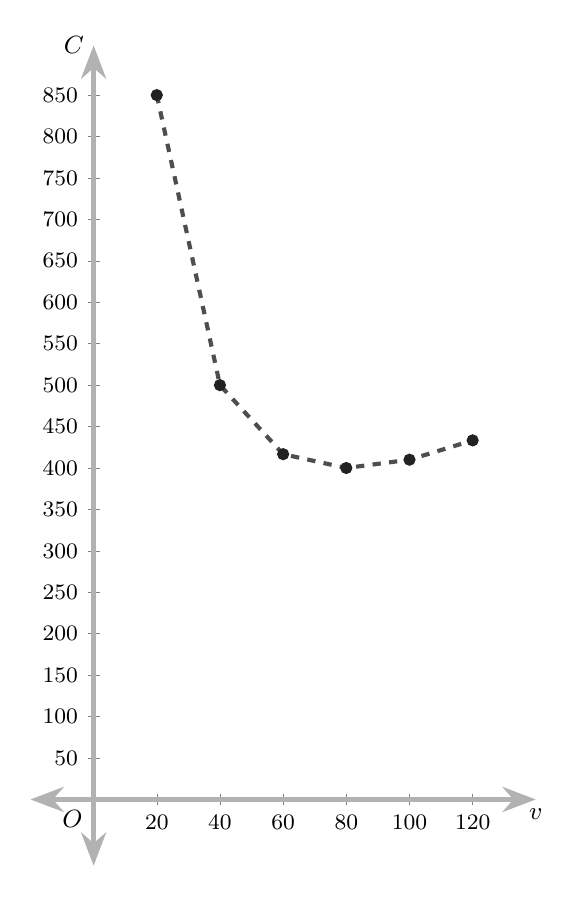
\begin{tikzpicture}
  \begin{axis}[
    axis lines = middle,
    axis line style={<->, line width=2pt, color=den-6!50},
    xlabel=$v$, ylabel=$C$,
    xlabel style={below, font=\small\sf},
    ylabel style={left, font=\small\sf},
    xmin=-20, xmax=140,
    ymin=-80, ymax=910,
    % restrict y to domain=0:10,
    width=8cm, height=12cm,
    xtick={20,40,60,80,100,120},
    xticklabels={$20$,$40$,$60$,$80$,$100$,$120$},
    % xtick style={draw=none},
    ytick={50,100,150,200,250,300,350,400,450,500,550,600,650,700,750,800,850},    
    yticklabels={$50$,$100$,$150$,$200$,$250$,$300$,$350$,$400$,$450$,$500$,$550$,$600$,$650$,$700$,$750$,$800$,$850$}, 
    % ytick style={draw=none},
    tick label style={font=\footnotesize\sf},
    clip=false,
    % yscale=2,
  ]

    \node[originlabel] at (axis cs:0,0) {$O$};

    % \addplot[domain=0:120, restrict y to domain=0:910, samples=200, line width=1.5pt, color=den-2, opacity=.8] 
    %     {16000/x+(5/2)*x};

    \addplot[dashed, line width=1.5pt, color=den-2, opacity=.8] coordinates {
        (20,850)
        (40,500)
        (60,416.67)
        (80,400)
        (100,410)
        (120,433.33)
        };    
    \addplot[only marks, mark=*, mark size=2pt, color=den-2] coordinates {
        (20,850)
        (40,500)
        (60,416.67)
        (80,400)
        (100,410)
        (120,433.33)
        };    
    % \addplot[dashed, line width=1.5pt, color=den-2, opacity=.8] coordinates {
    %     (120,0)
    %     (120,433)
    %     };    
  \end{axis}
\end{tikzpicture}

\end{document}
